\section{Results}

The results of the project are best understood as the final achieved behaviour of the implemented Micromouse system after the testing and tuning process described in the previous chapter. For this reason, the present section does not repeat the validation procedures in detail, but instead summarizes the final technical outcomes of the sensing, control, and navigation development. Overall, the project resulted in a functioning autonomous robot that was able to combine wall detection, closed-loop motion control, and map-based maze traversal in a single embedded platform.

\subsection{Sensor Results}

The infrared sensing system produced reliable wall-detection signals that were suitable for both control and navigation tasks. In practical operation, the most important outcome was not the exact reconstruction of metric wall distance, but the dependable distinction between the presence and absence of nearby maze walls. For this purpose, a sensor value of $800$ proved suitable as the final wall-detection threshold. This made it possible to use the side sensors for wall-based trajectory correction and the front sensor for front-wall detection and cell interpretation.

The sensor measurements also showed that the practically relevant operating range inside the maze was smaller than the full nominal range suggested by the datasheet. In free measurements, raw values reached approximately $3300$, whereas in realistic maze conditions the side sensors reached only about $2300$ at very close wall distances. Nevertheless, the available signal range was fully sufficient for the implemented purpose. As a result, the sensing subsystem can be regarded as successful, since it provided stable and usable input signals without requiring major redesign.

\subsection{Controller Results}

The drive controller achieved stable closed-loop wheel-speed regulation and sufficiently accurate straight-line motion for the intended maze task. After tuning, the final wheel-speed controller operated with the parameter values $K_P = 1.4$ and $K_I = 16.0$ at a sampling time of $T_s = 0.01\,\mathrm{s}$. The same PI parameter set was used for both wheels, since this provided sufficiently similar behaviour on the left and right side while keeping the implementation simple. As summarized in Appendix~A, lower proportional gains produced little visible regulating effect, whereas substantially higher gains led to increasingly irregular and stuttering behaviour; the selected final parameters therefore represented the most useful compromise observed during empirical tuning. With these settings, the motors tracked commanded speeds reliably enough for repeated straight driving and for the execution of the higher-level navigation functions.

In addition to the inner wheel-speed loop, the wall-based outer correction layer produced a clear practical improvement in corridor tracking. The final implementation used a proportional trim controller with gain $K_P = 0.004$, because this gave better behaviour than the initially considered PI-based trim correction. In practice, the proportional correction avoided the pronounced oscillatory motion observed previously and provided a more direct and stable correction of lateral deviations. The final implementation applied wall-based correction only when a valid side-wall reference was available, used a target side-sensor value of $1130$, and employed low-pass filtering with $\alpha = 0.50$ for the measured wheel speed and $\alpha = 0.30$ for the trim signal. In addition, the drive command was slew-rate limited to a maximum change of $0.07$ per control step. Together, these measures led to sufficiently smooth drive behaviour for maze operation. The final default drive speed of the implemented system was $500\,\mathrm{mm/s}$.

\subsection{Navigation Results}

The final navigation software was able to combine local sensor-based decisions with a persistent internal maze representation. In operation, the robot could detect cell transitions, store neighbouring cell connections, and maintain a consistent orientation estimate sufficiently well for incremental exploration of the reduced $6 \times 6$ maze. This confirmed that the combination of encoder-based distance estimation and front-sensor-based cell interpretation was adequate for the reduced project scope.

After the exploration phase, the robot was able to use the generated map for purposeful movement through already explored maze regions. In particular, the implementation was capable of returning after exploration and, on the following run, using the stored map to calculate and follow a path toward the predefined goal. The navigation result is therefore significant not because the system achieved maximum speed, but because it demonstrated the complete functional chain from sensing and control to localisation, mapping, and goal-directed motion.

Figure~\ref{fig:robot_in_maze} shows the Micromouse inside the reduced test maze during operation. This image is worth including because it documents the final integrated system in its actual environment and gives the reader a direct impression of the physical scale and testing context of the achieved navigation behaviour.

\begin{figure}[t]
    \centering
    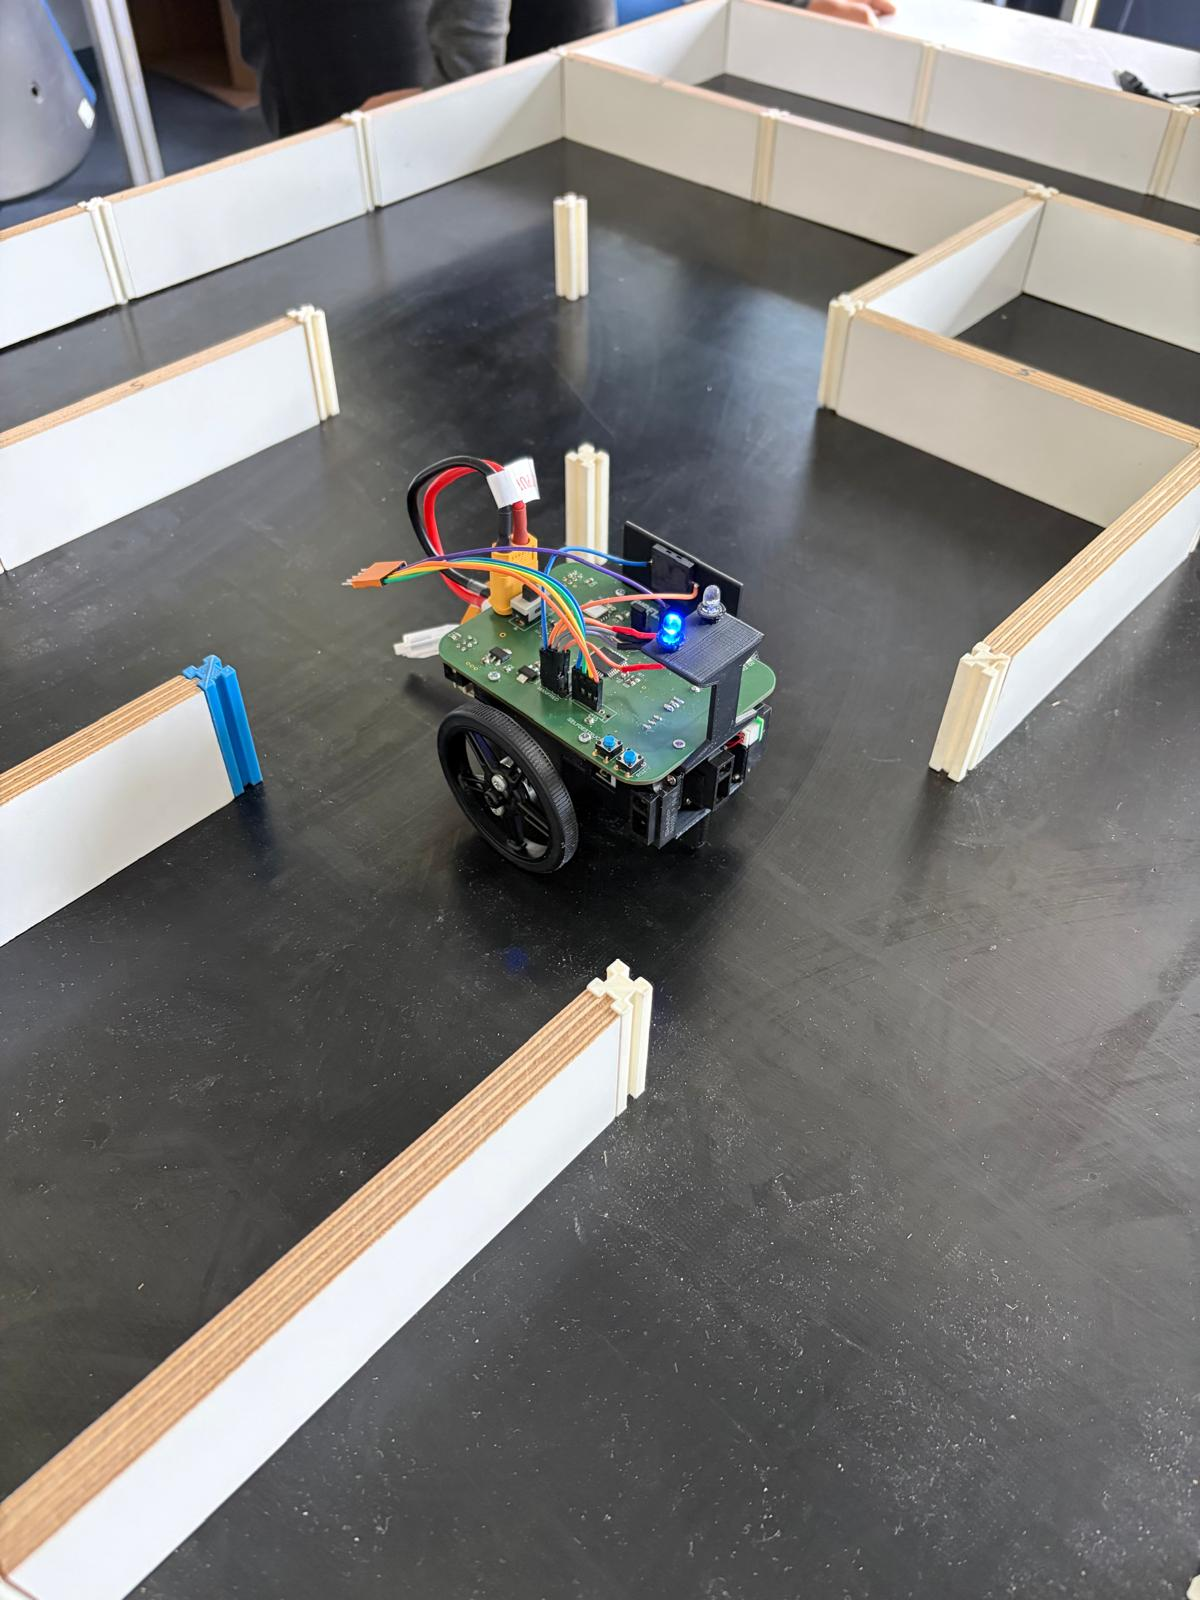
\includegraphics[width=0.82\columnwidth]{images/robot_and_maze.jpeg}
    \caption{Micromouse operating inside the reduced test maze.}
    \label{fig:robot_in_maze}
\end{figure}

\subsection{Overall System Result}

Taken as a whole, the project achieved its primary goal of producing a functioning Micromouse prototype that integrates electronics, embedded software, control, and navigation in one system. The robot was able to detect maze walls, regulate its wheel motion in closed loop, explore a reduced maze representation, and reuse the generated map for a later goal-directed run. This confirms that the implemented concept was technically viable and that the selected architecture was appropriate for the intended task.

At the same time, the results also show the limits of the current implementation. The realised platform should be understood as a functional academic prototype rather than as a fully competition-optimised high-speed Micromouse. Nevertheless, within the intended scope of the project, the achieved behaviour demonstrates that the essential design objectives were met and that the robot operated successfully as an autonomous embedded navigation system.
